\chapter*{Spis załączników}
\addcontentsline{toc}{chapter}{Spis załączników}
\noindent

\begin{tabularx}{\textwidth}{Xl}

    Pełny schemat bazy danych & str. \pageref{file:database-schema} \\

    Pełny opis zadania projektowego dla przedmiotu ”Podstawy Programowania” w realizacji zima 2018 & str. \pageref{file:penguins_description} \\

    Definicja przypadków testowych dla symulacji projektu historycznego & str. \pageref{file:test_cases_penguins} \\

    Definicja przypadków testowych dla symulacji projektu z operacjami na macierzach & str. \pageref{file:test_cases_matrix} \\

\end{tabularx}

\chapter*{Załączniki}
\addcontentsline{toc}{chapter}{Załączniki}

%%%%%%%%%%%%%%%%%%%%%%%%%%%%%%%%%%%%%%%%%%%%%%%%%%%%%%%%%%%%%%%%%%%%%%%%%%
\section*{Pełny schemat bazy danych}
\label{file:database-schema}
{
\tiny
\verbatiminput{back//platform_schema.sql}
}

%%%%%%%%%%%%%%%%%%%%%%%%%%%%%%%%%%%%%%%%%%%%%%%%%%%%%%%%%%%%%%%%%%%%%%%%%%
\section*{Pełny opis zadania projektowego dla przedmiotu ”Podstawy Programowania” w realizacji zima 2018}
\label{file:penguins_description}
{
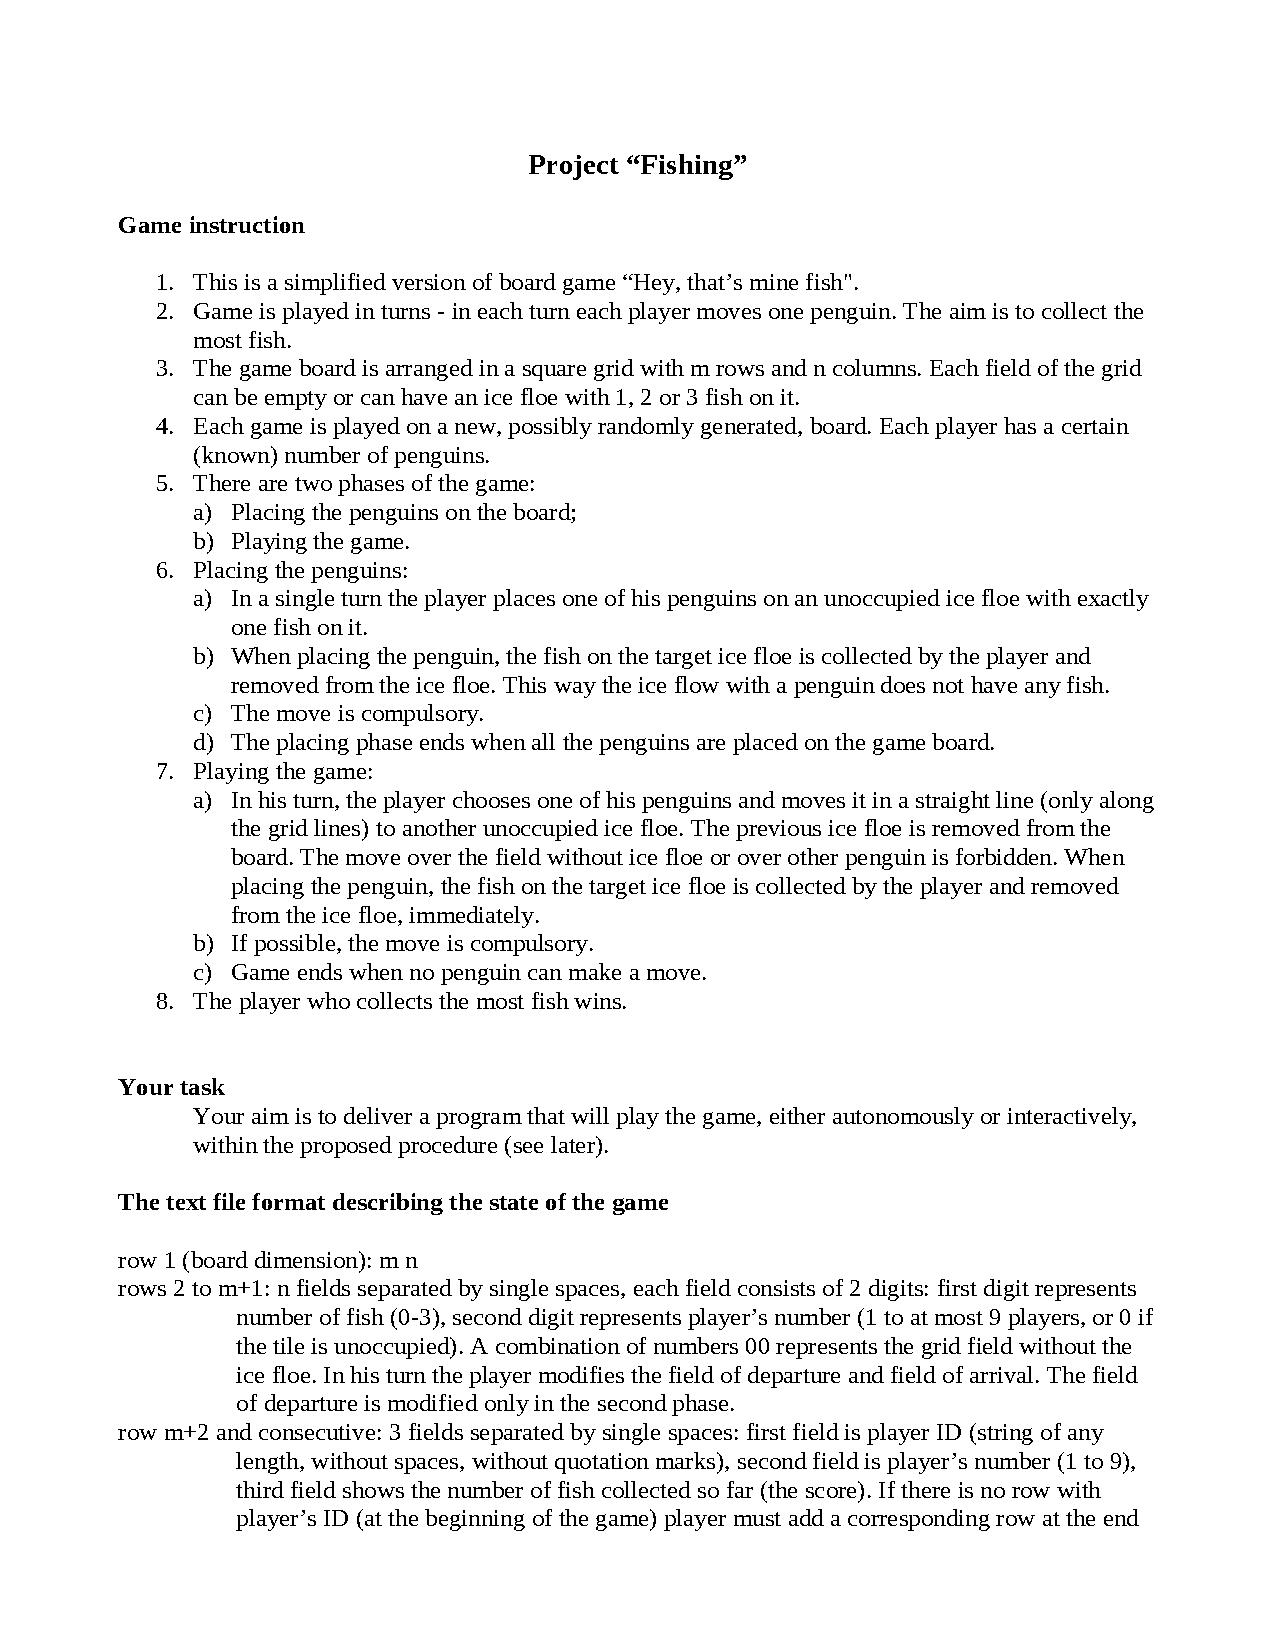
\includepdf[page={1,2,3,4}]{back//penguins_description}
}


%%%%%%%%%%%%%%%%%%%%%%%%%%%%%%%%%%%%%%%%%%%%%%%%%%%%%%%%%%%%%%%%%%%%%%%%%%
\section*{Definicja przypadków testowych dla symulacji projektu historycznego}
\label{file:test_cases_penguins}

{
TODO: Insert
}

%%%%%%%%%%%%%%%%%%%%%%%%%%%%%%%%%%%%%%%%%%%%%%%%%%%%%%%%%%%%%%%%%%%%%%%%%%
\section*{Definicja przypadków testowych dla symulacji projektu z operacjami na macierzach}
\label{file:test_cases_matrix}

{
TODO: Insert
}


\clearpage
